\subsection{UC9: Esportazione di un grafico.}
\label{sub:uc9}

%TODO aggiornare caption con nome più preciso
\begin{figure}[h]
    \centering
    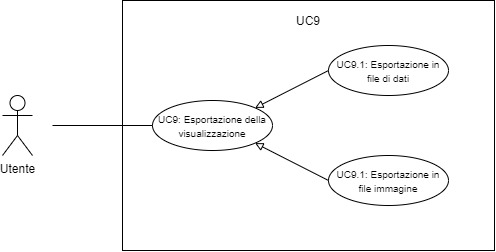
\includegraphics[width=0.5\textwidth]{componenti/casi-duso/diagrammi/UC9.jpg}
    \caption{UC9 - }
    \label{fig:UC9}
\end{figure}


\begin{itemize}
    \item{\textbf{Descrizione}}: L'utente effettua l'esportazione del risultato di un'elaborazione HD Viz una volta visualizzata;
    \item{\textbf{Attore primario}}: Utente;
    \item{\textbf{Precondizione}}: L'utente ha scelto una tipologia di grafico e lo ha visualizzato (UC7);
    \item{\textbf{Postcondizione}}: La configurazione attuale di HD Viz viene esportata sul sistema dell'utente;
    \item{\textbf{Scenario principale}}:
    \begin{enumerate}
        \item   L'utente visualizza l'elaborazione dei dati su HD Viz;
        \item   All'utente viene proposto di esportare un file contenente i dati oppure 
                di effettuare una cattura ad immagine della visualizzazione corrente;
        \item   L'utente seleziona l'opzione desiderata;
        \item   I dati o il progetto vengono esportati nella modalità scelta dall'utente.
    \end{enumerate}
    
    \item{\textbf{Generalizzazioni}}: L'utente seleziona la modalità:
    \begin{enumerate}
        \item   Esportazione come file di dati (UC9.1);
        \item   Esportazione come file immagine (UC9.2).
    \end{enumerate} 
\end{itemize}

\subsubsection{UC9.1: Esportazione in file di dati}
\begin{itemize}
    \item{\textbf{Descrizione}}: L'utente effettua l'esportazione dei dati da elaborati da HD Viz come file di dati;
    \item{\textbf{Attore primario}}: Utente;
    \item{\textbf{Precondizione}}: L'utente ha visualizzato il grafico elaborato da HD Viz;
    \item{\textbf{Postcondizione}}: La struttura del grafico viene esportata nel sistema dell'utente;
    \item{\textbf{Scenario principale}}: L'utente seleziona l'opzione di esportare come file di dati da HD Viz.
\end{itemize}

\subsubsection{UC9.2: Esportazione in immagine}
\begin{itemize}
    \item{\textbf{Descrizione}}: L'utente effettua l'esportazione dei dati elaborati da HD Viz come "cattura immagine" della visualizzazione corrente;
    \item{\textbf{Attore primario}}: Utente;
    \item{\textbf{Precondizione}}: L'utente ha visualizzato il grafico elaborato da HD Viz;
    \item{\textbf{Postcondizione}}: La visualizzazione corrente del grafico viene esportata nel sistema dell'utente come file immagine;
    \item{\textbf{Scenario principale}}: L'utente seleziona l'opzione di esportare come immagine da HD Viz.
\end{itemize}
